\chapter{RNA Base Steps}
\label{basesteps} 
\bibliographystyle{nar}
The problem of classification of the space of conformations
% configurations? 
of  RNA is  not new,  see  for example,  Olson 1972  \cite{olson1972},
Saenger     1984     \cite{saenger1984},     and    Gautheret     1993
\cite{gautheret1993}.  This problem  had  only been  addressed by  a few
researchers before the  turn of the twenty first century,  but starting in
the year 2000  a vast amount of RNA  structural information has become
available  with the  elucidation of  the  structure of  the 30S  small
ribosomal  subunit  of   \textit{Thermus  thermophilus},  a  bacterial
ribosome   \cite{wimberly2000,schluenzen2000},  and   the   50S  large
ribosomal subunit of \textit{Haloarcula marismortui}, an archaeal
\footnote{I emphasize the  phylogeny of rRNA's here since  there is an
  ongoing discussion among biologists on whether archaea are  closer
  to prokaryotes, or to eukaryotes.}  ribosome \cite{ban2000}.

\begin{figure}[H]
\centering
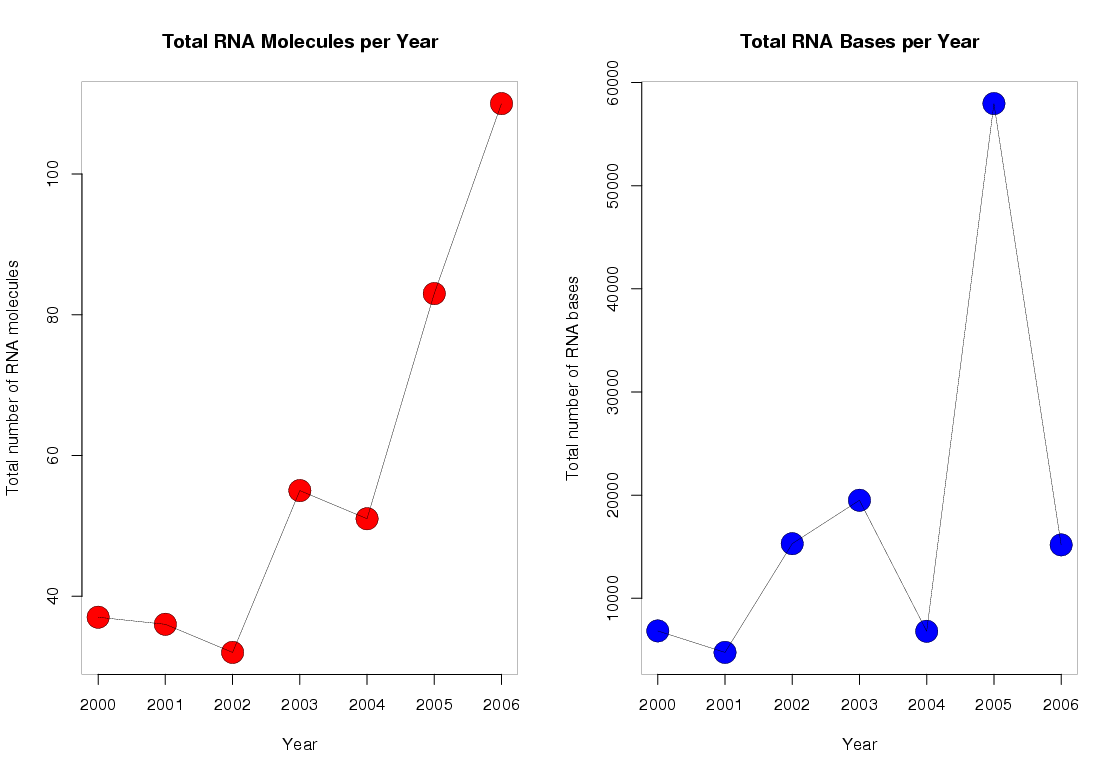
\includegraphics[scale=0.4]{Chapter2/rna_per_year.png}
\caption{\textbf{Left:} Total number of RNA structures solved yearly by X-Ray 
crystallography between 2000 and 2006. \textbf{Right:} Total number of 
RNA bases added to the PDB database between 2000 and 2006.}
\label{fig:rnainpdb}
\end{figure}

\noindent Between  1972 and  2000 a total  of 132 RNA  structures with
resolution greater  than 3 \AA, and comprising  around 5500 nucleotide
bases were found  in the Protein Data Bank (PDB),  and between 2000 and
today  a  total of  460  RNA\index{RNA}  structures comprising  around
140000  nucleotide   bases  have been  found.  That  is,   the  increase  in
information  due to  the solution of large RNA  structures  is two orders  of
magnitude as pointed out  by Noller \cite{noller2005} in 2005. Looking
at the growth of RNA structural information from 2000 until today it's
important  to  point  out  that,  although the  total  number  of  RNA
structures  deposited in the  PDB shows  exponential growth  (see left
panel in  Figure~\ref{fig:rnainpdb}), the total number  of RNA bases 
does not show a well defined trend (see right panel in
Figure~\ref{fig:rnainpdb}). 
This is due to the
size preponderance of ribosomal  structures. That is, in 2005 nineteen
ribosomal structures were  deposited in the PDB, whereas  in 2006 only
four  were deposited.  So, even  though interest  in RNA  seems  to be
growing  since  ribosomal structures  have become  available  in 2000,  and
two Nobel  prizes were awarded for work in  RNA in 2006, along
with  the  exciting  possibilities  of  deciphering  even  larger  RNA
virus\index{virus} structures, still the  growth of the RNA structural
field is  far from that  of proteins if  weighed by the growth  of RNA
structural information in  the past seven years. This  fact might just
be due to the smaller  sizes and structural diversity of RNA molecules,
which,  as can  be seen  in Figure~\ref{fig:rnaranges}, is  restricted  to
``compact'' nucleotide ranges\index{RNA!ranges}.
%\footnote{One can
% also think of another range of even larger viral RNA's \cite{heitsh}, and yet
%another one of nanodesgined RNA's \cite{shapiro, orland}}. 
A representative example of these  characteristic ranges can be seen in
Table 1.1 for structures larger than 300 bases.

\begin{figure}[H]
\centering
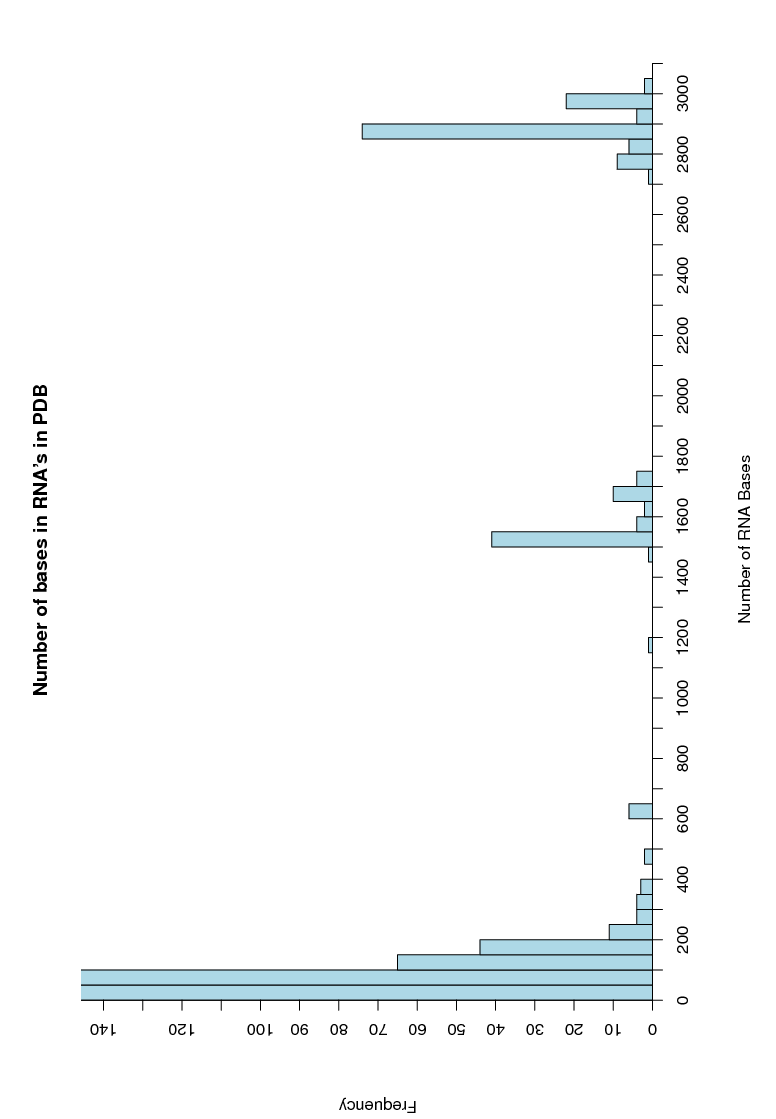
\includegraphics[scale=0.60]{Chapter2/histogram.png}
\caption{Frequency of nucleotide bases in RNA molecules found in the
  PDB classified by the size of RNA molecules. We define the size as the
  total number of nucleotide bases present per molecule.}
  \label{fig:rnaranges}
\end{figure}
%The table and Figure 1.1 come from downloading all structures from
%2000, until today that have RNA in the pdb and that have a resolution
%better that 3.0A, they are 460 structures.

\noindent Analysis of RNA conformational information contained in this
structural data can  be divided into three main  perspectives: an atom
based perspective; a bond  based perspective; and a third, as yet unexplored
to our knowledge,  rigid-body based perspective.   In the atom based
perspective,  either direct  comparison of  backbone atom  positions is
made \cite{reijmers2001}, or a comparison of distances between a reduced
set  of atoms  taken from  the  nucleotide backbone,  sugar, and  base
\cite{sykes2005}. The bond based  perspective is divided into three main
categories; the first considers the consecutive covalent bonds in the RNA
backbone and the glycosidic bond between the sugar and base,  that is, six
backbone   torsion   angles   and   one   glycosidic   torsion   angle
\cite{reijmers2001,  murray2003, hershkovitz2003, schneider2004,
hershkovitz2006};
or alternatively the pseudo-bonds between consecutive
P and  C4$\prime$ atoms  and the resulting  pseudo-torsion angles  $\eta$ and
$\theta$  \cite{olson1972,  duarte1998,  duarte2003, wadley2007}.  The
third category considers the  networks of horizontal hydrogen bonding
patterns coming  from a definition  of interacting edge  boundaries in
the nucleotide bases  \cite{westhof2000, leontis2002, leontis2006}. In
this report we review one category of the bond based
perspective. Namely we review the  case where the covalent bonds
between backbone atoms give rise to torsion angle space. We also make
a first study of the rigid body based perspective using clustering analysis.
\begin{table}[htbp]
\begin{center}
{\small
\begin{tabular}{c|p{5cm}|c|c|c}
\hline
\bf{PDBID} & \bf{Structure Name} & \bf{Phylogenetic Group} & \bf{Number of bases} & \bf{Year} \\ \hline
1l8v & Mutant of P4-P6 Domain of Group I Intron & Eukaryote & 314 & 2002 \\ \hline
1fg0 & Central Loop in Domain V of 23S rRNA & Archaea & 499 & 2000 \\ \hline
2nz4 & GlmS Ribozyme & Eukaryote & 604 & 2006 \\ \hline
1xmq & 30S rRNA & Bacteria & 1522 & 2004 \\ \hline
1ffk & 50S rRNA Subunit & Archaea & 2828 & 2000 \\ \hline
\end{tabular}
}
\caption{Some large RNA structures ($>$300 bases) elucidated in the last 7 years.}
\end{center}
\end{table}

\section{Dinucleotide   Torsion  Angles}   The  covalent   bond  based
perspective as  mentioned in  the previous section  gives rise  to six
backbone  torsion  angles  and  one  glycosidic  torsion  angle.  This
heptaparametric space  has been the subject of  several recent studies
of    RNA   dinucleotide    steps.   Richardson    and   collaborators
\cite{murray2003}  have   applied  van  der   Waals  radius  filtering
techniques on a database of  8636 nucleic acid residues from RNA X-Ray
structures  with  resolution  of  3.0  $\AA$ or  better  grouping  all
structures in 42 conformers which they refer to as rotamers. Berman et
al. \cite{schneider2004}  reduced the data space of  the large subunit
of   the  \textit{Haloarcula   Marismortui}  ribosome   using  Fourier
transform filtering. Hershkovitz et al. \cite{hershkovitz2003} defined
lower and upper  bounds of torsion angle values  by ``binning'' in one
dimension. Pyle  et al. \cite{wadley2007}  reduced the heptaparametric
space  to  a  biparametric   one,  defining  a  virtual  bond  between
consecutive O and C4$\prime$ atoms in the RNA backbone.

Hershkovitz and collaborators \cite{hershkovitz2006} took a first
step towards integrating clustering  analysis formally in the study of
RNA  backbone torsion  angles. In  particular, they  used  the k-means
partitional  clustering algorithm. \footnote{For  a reason  that still
eludes  the author,  instead of  using  the more  general and  familiar
terminology  of clustering  analysis,  they refer to  this
method as if it was not a clustering analysis method. In one case they
call their method scalar quantization, when one torsion angle
at a time is clustered. They call it vector
quantization when they want to cluster groups of more than one torsion
angle  at a time.}   It's important  to note  that Hershkovitz  et al.
reduce the  data set  of all torsion  angles in rRNA's  large subunit,
using their binning approach prior to k-means clustering.

Clustering analysis  can be divided into two  main methodologies,
namely,  hierarchical    clustering   and    partitional    clustering
\cite{jain1999}. We  have used particular cases  of both methodologies
to  investigate  thoroughly  if  ``biased'' \footnote{By  biased  data
reduction we  mean that a reduction of  the whole data set  is done by
taking into account a particular bias  imposed by us. This bias can be
structural or sequence  based.}  data reduction is needed,  as has been
suggested by various authors \cite{schneider2004, hershkovitz2006}, or
if the  use of  clustering analysis alone  can be  used to find  in an
efficient and  clear manner subsets of RNA  conformational space which
possess a clear structural meaning.

\subsection{Partitional Clustering for Torsion Angles}
For  partitional clustering the k-means  algorithm as
implemented  in  the  software  package  \textbf{R}  \cite{Rproj} was employed.
\footnote{Another
partitional algorithm that could readily be used in the future is pam (partitioning  around medoids). For now we've determined
the average silhouette width, which is an analogous quantity
to the average distortion \textbf{D}, (which will be defined later in 
the text) and plotted this value against the number of clusters as can
be seen in Figure~\ref{fig:asw}}

We consider the  2753 base-steps  of the 23S  subunit of the  ribosome as
vectors  of  seven dimensions  composed  of  the previously  mentioned
backbone  torsion   angles  $\alpha$,  $\beta$,   $\gamma$,  $\delta$,
$\epsilon$,  $\zeta$, and  the  glycosidic torsion  angle $\chi$.  The
\textbf{R}  software  package has  implemented  four different  k-means
algorithms; \textit{Hartigan-Wong};   \textit{Lloyd};
\textit{Forgy}; and \textit{MacQueen}. For the data set used, that is,
the  large subunit  of the  ribosome  (PDB code  1jj2), no  noticeable
differences were  found with the four k-means
algorithms when we group  the data into two partitions, as can
be seen in Figures~\ref{fig:hartigan} through~\ref{fig:macqueen}.

%The Figures for the different types of k-means used to go here.

One of the problems with k-means  is that the number of clusters is not
an emergent property  of the data set but  a parameter that has
to  be given  to the  algorithm. This  problem has  been given  a good
amount of attention in the statistical analysis community, in the area
of clustering  analysis. Hershkovitz  et al. \cite{hershkovitz2006} 
use  one method  which is
common in clustering analysis and  find a so-called distortion measure
\textbf{D}, also called the ``within clusters sum of squares'' in the more
common  clustering analysis  area. That  is, the squares of the
elements of each cluster is found and then added. This quantity can be plotted
against the number of clusters k that were selected as can be seen in
Figure~\ref{fig:wss}. The ``optimal''  number of clusters corresponds
to the value of k where \textbf{D} becomes constant,  which in
Figure~\ref{fig:wss} is
around 60. Where interestingly  Figure\ref{fig:wss}  is very
similar to Figure 8 in the paper of Hershkovitz et al.
\cite{hershkovitz2006}, where the \textbf{D} value becomes constant
also around 60.  The main
difference  between our  plot and  theirs is  that they  exclude
dinucleotide steps  which are close  to the A-type  conformation. They
further state  that the A-type steps amount to  over 60$\%$ of  the data, meaning
that  the   remaining  40$\%$  accounts   for  the  majority   of  the
conformational diversity  of the space of torsion  angles, since there
is  not a  significant change  in the  value where  \textbf{D} becomes
constant.
%The reference for this quantity is Everitt and Hothorn (pg. 251).

There are more  methods to determine the optimal  amount of partitions
that a data set can be split into. For example, one can also do another
partitioning around  medoids (PAM), and  find an analogous quantity
to the within  clusters sum of
squares, such quantity is called the average silhouette width, and the
optimal number of  clusters is that which maximizes  this quantity. In
Figure~\ref{fig:asw} we can see that the maximum corresponds to $k=3$,
nonetheless, we also see various local maxima, for example in $k=16,
22, 28, 31, 36, 45, 48, 51, 57$, it's interesting to point out that in
a very recent preprint by  Berman et al. \cite{richardson2008} they review
the work on RNA backbone  conformations and summarize that different 
research groups find 32, 37, and 42 discrete RNA conformations.

Another way of  selecting k is just by visual  inspection of the data.
In   our   case   if   we    take   any   of   the   scatterplots   in
Figures~\ref{fig:hartigan}  thru~\ref{fig:macqueen},  we  can  imagine
that  in some  of them  the data  seems to  be clustered  around eight
groups\footnote{Checking the  data in  two dimensions more  clearly it
seem to me that  at most one could say that there  can be six groups}.
We choose eight groups also because this is the result that Duarte and
Pyle  obtain  for their  classification  based  on RNA  pseudotorsions
\cite{duarte1998}.
%It would be interesting to explore further if such groups are similar
%structurally to the eight clusters which can be seen clearly in Duarte
%and Pyle's
%$\theta$ vs. $\eta$ pseudotorsion angle plots \cite{duarte1998}.
Following this  argument we  can color code  our scatterplots  for the
cases  where we  select k  to be  eight and  sixty as  can be  seen in
Figures~\ref{fig:k8} and~\ref{fig:k60}.  In Figure~\ref{fig:k8} we see
that for  k=8, the  k-means method clearly  does not  differentiate the
clusters as one would expect, that  is, one might expect to find eight
clearly separate color  regions for the $\zeta$ vs  $\alpha$ plot, but
we see that they overlap too much, this should not be surprising since
we are just looking at  the projections of a heptadimensional space in
a bidimensional one. We have also plotted the cluster centers as black
dots of greater  diameter and we see that  the cluster centers overlap
in three  separate regions. For Figure~\ref{fig:k60} the  case is even
more  confusing  since one  would  have  to  distinguish 60  different
colors. This  situation doesn't get  better when instead of  colors we
use numbers from  one thru sixty to show which  points belong to which
cluster.  The  previous  results  are  a good  argument  to  use  data
reduction approaches,  we propose to  introduce biased classifications
on the data,  whether the bias has its origin  in taking sequence into
account,   or  from   chemical  considerations   like   taking  A-type
conformations into account, for  example, more interesting results can
be  obtained as has  been shown  by others  \cite{hershkovitz2006}. 
%We
%have yet to start taking  into account sequence classification for the
%case of  the heptaparametric torsion  angles space, but  we've already
%started to do for the case of  the rigid-body base-step parameters
%as will be seen later in this review.

\begin{figure}[H]
\centering
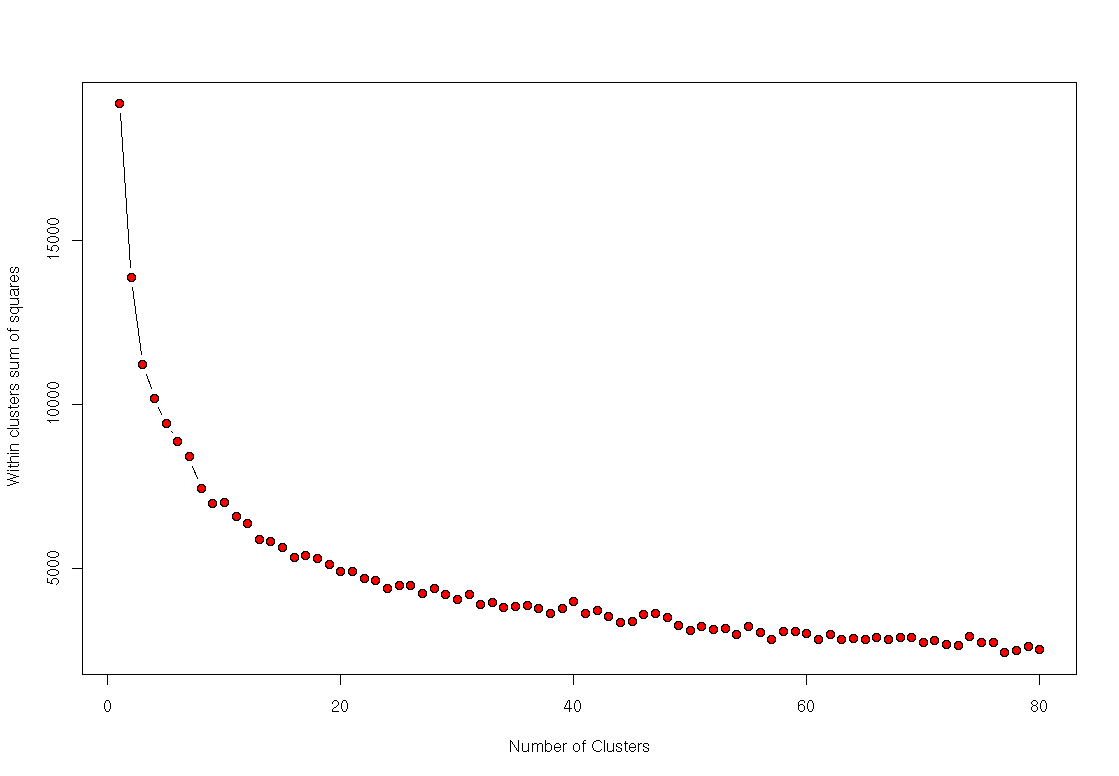
\includegraphics[angle=0, scale=0.35]{Chapter2/hartigan_nuclu_b.png}
\caption{Sum of all within clusters sum of squares against number of 
 clusters for data of all torsion angles in 23S rRNA.}
\label{fig:wss}
\end{figure}

\begin{figure}[H]
\centering
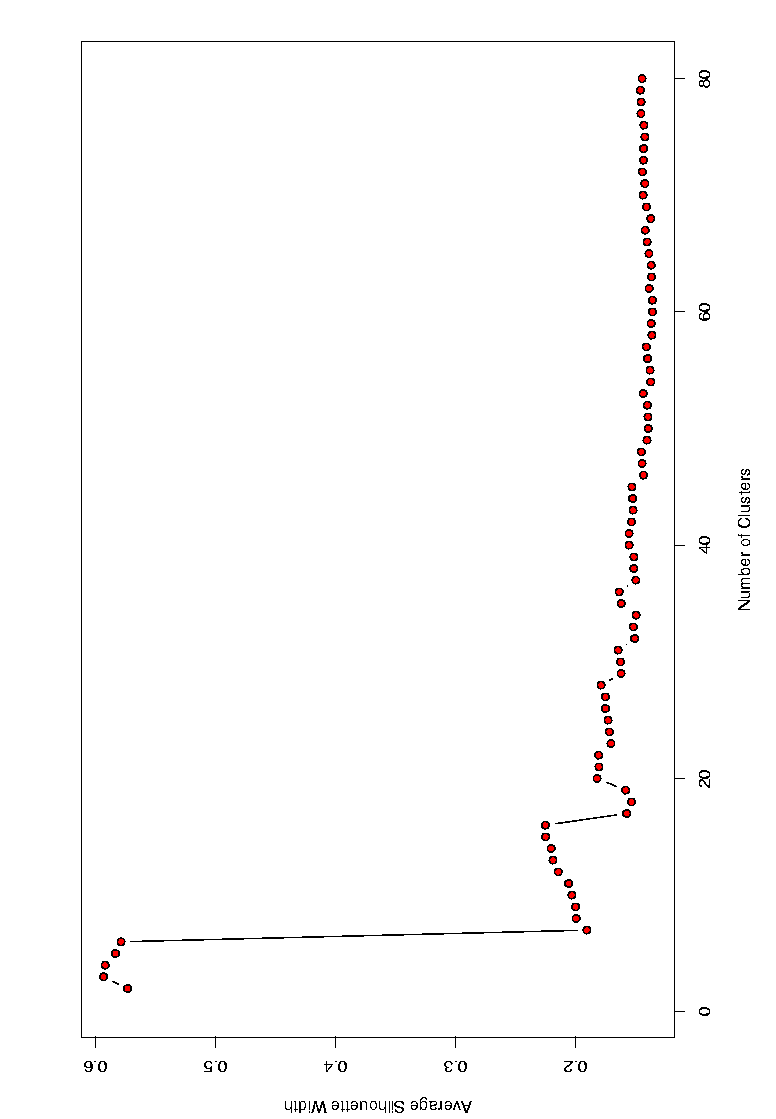
\includegraphics[angle=270, scale=0.48]{Chapter2/pam_asw_2_80_torsions.png}
\caption{Average silhouette width against  number of clusters for data
of  all torsion angles  in 23S  rRNA. The  best clustering  method and
value of $k$ is then defined as the model that maximizes a.s.w.}
\label{fig:asw}
\end{figure}

\begin{figure}
 \centering
 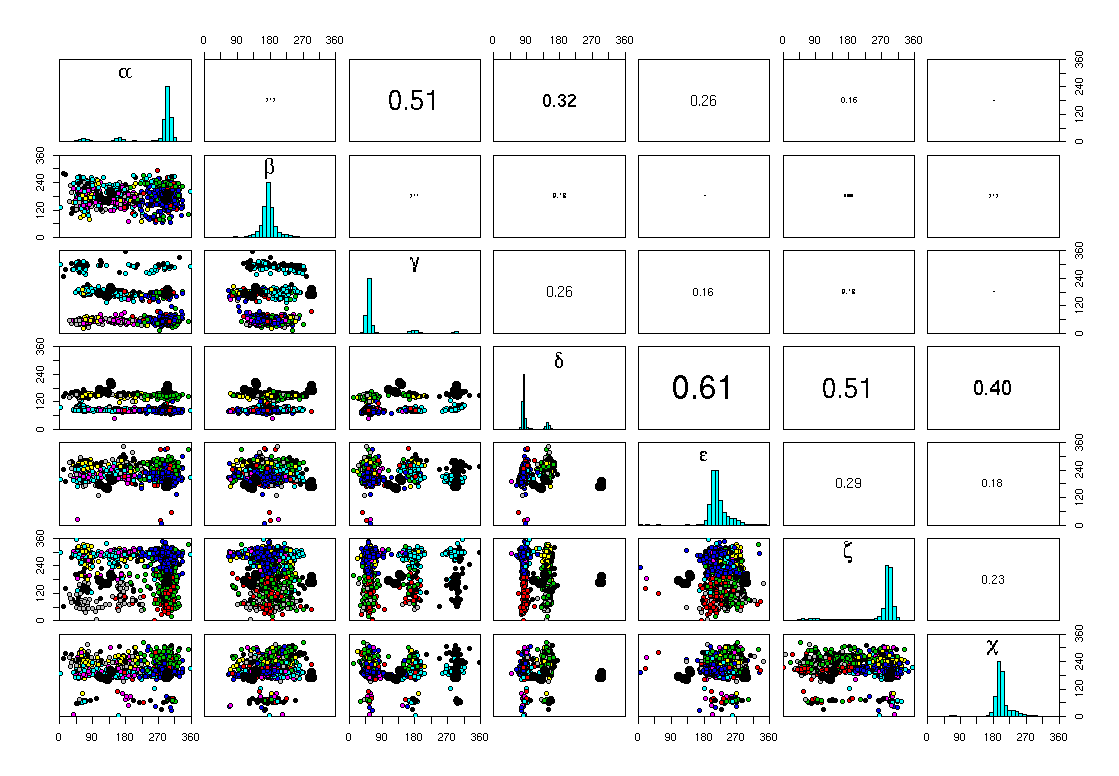
\includegraphics[angle=90, scale=0.50]{Chapter2/hartigan_k8_b.png}
 \caption{K-means clustering of  heptadimensional torsion angle vectors
of  2753  dinucleotide  steps  present  in 23S  rRNA.  The  number  of
partitions  is  \textbf{8}.  The  large  black  dots  represent cluster
centers. The upper diagonal matrix displays the values of the linear
correlation coefficient $r$, and a histogram showing the torsion angle
distribution is rendered in the diagonal.}
 \label{fig:k8}
 \end{figure}
 
\begin{figure}[htbp]
 \centering
 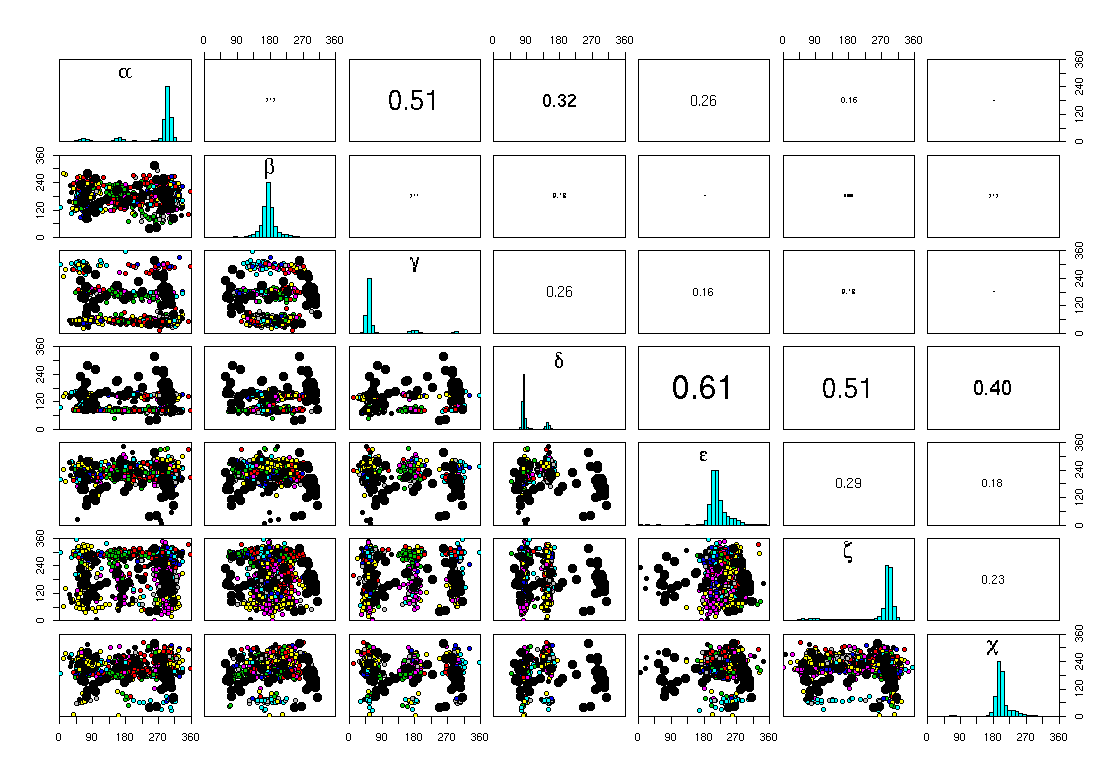
\includegraphics[angle=90, scale=0.50]{Chapter2/hartigan_k60_b.png}
 \caption{K-means clustering of  heptadimensional torsion angle vectors
of  2753  dinucleotide  steps  present  in 23S  rRNA.  The  number  of
partitions  is  \textbf{60}.  The  large  black  dots represent cluster
centers. The upper diagonal matrix displays the values of the linear
correlation coefficient $r$, and a histogram showing the torsion angle
distribution is rendered in the diagonal.}
 \label{fig:k60}
 \end{figure}

\begin{figure}[htbp]
 \centering
 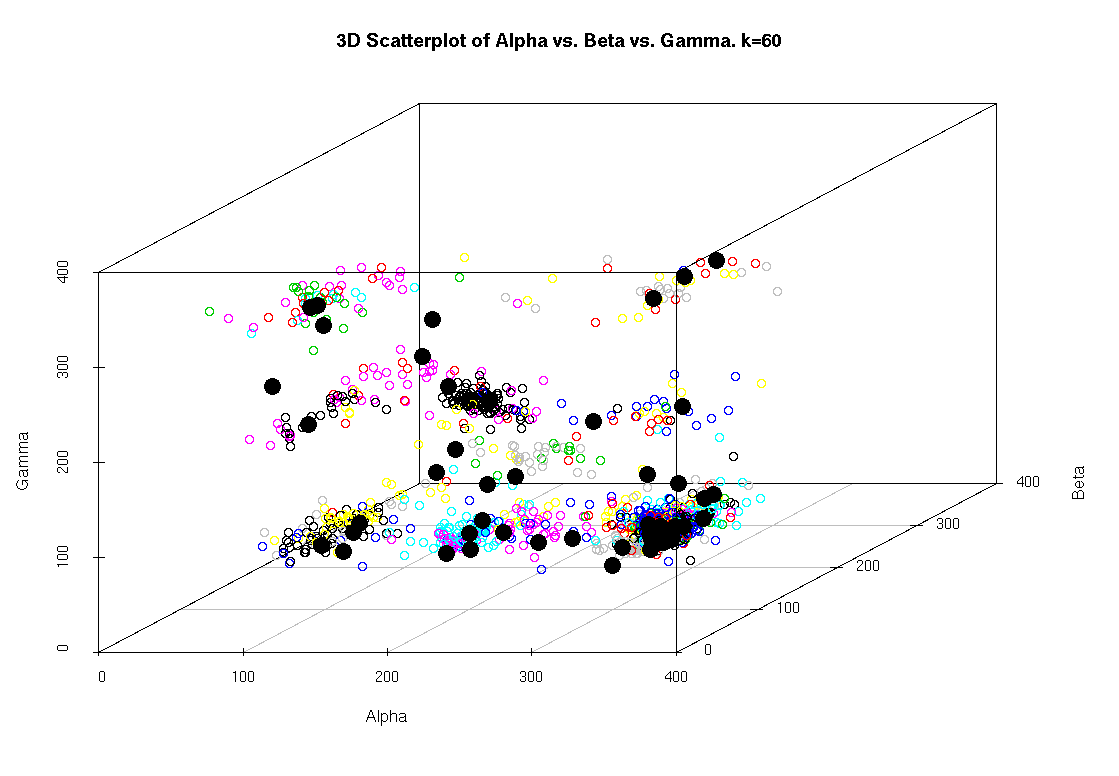
\includegraphics[angle=90, scale=0.50]{Chapter2/hartigan_k60_3D_b.png}
 \caption{K-means  clustering  of  the heptadimensional  torsion  angle
vectors of 2753 dinucleotide steps of  23S rRNA. The axis of the three
dimensional scatterplot  corresponds to the  torsion angles, $\alpha$,
$\beta$,  and $\gamma$.   The  large black  dots  correspond with  the
cluster centers for clustering by using k-means with k=60.}
 \label{fig:3d}
\end{figure}


\subsection{Hierarchical Clustering for Torsion Angles}
Other  authors have  used hierarchical clustering  to analyze the
torsion angles in nucleic acid structure, taking the Fr\"{o}benius
norm and Ward's method as the distance definition
for   four   different    RNA   representations   (see   Reijmers   et
al.  \cite{reijmers2001}) on  a ``small''  database similar to that of
Duarte and Pyle  \cite{duarte1998}. This  databases  do not
include ribosomal RNA's. The other  case where hierarchical clustering
has been used  did not  use torsion  angles, but rather a set  of  15 atoms
belonging  to the  nucleotides sugar  and  backbone. The latter study
used used  the unweighted pair  group method  (UPGMA) to classify  a database  of RNA
loop structures (see Huang et al. \cite{huang2005}).

In our case we  used three distance definitions (Euclidean, Manhattan,
and maximum),  and four  different clustering methodologies,  that is,
single, complete, average  and centroid (see~\ref{appendix_a}. We tried to  make a consensus
analysis of the twelve trees  obtained, but these trees are too large.
The number of trees, that is, twelve, is also too small compared with
the data vectors (2753 step vectors), for  the algorithms to find a  reasonable consensus. 
We were not even able  to find consensus for two  ``near'' clusters, where the
``near''  criteria  was  taken   from  a  tree dissimilarity algorithm
implemented in  \textbf{R}  cluster and   whose   result   can    be   
seen   in Figure~\ref{fig:clusdissim} where the previously mentioned 
``near'' clusters refer to clusters five and nine.  
One  typical  suggestion  in  clustering
analysis is to just use the  single linkage method since this one uses
as  its  grouping  criteria  the minimal  distance  between  clusters,
therefore giving a direct interpretation of the trees as just a direct
minimal  proximity   relation  depending  on  the   metric  being used
(see Appendix~\ref{appendix_a}). \footnote{The  author still has to  do
consensus of single  method trees.}  In  Figure~\ref{fig:hclus} we
see twelve
clustering trees clustering all base-steps in the large subunit of the
ribosome. It's noticeable that trees are more similar  when the linkage
method is the same than when the metric is the same. The main problem 
with the dendrograms in Figure~\ref{fig:hclus} is very similar to that 
of determining the number of partitions in partitional clustering. In
this case we have to determine which is the optimal tree height which 
would determine how many meaningful groups we have, for 
Figure~\ref{fig:hclus} we have selected to draw boxes around a group of 
branches at the height where 36 branches are found. The reason for 
selecting 36 is because this was one of the maxima in Figure~\ref{fig:asw}
and because it´s close to 37, the number of discrete nucleotide conformations
suggested by Hershkovitz et al. \cite{hershkovitz2006}

\begin{figure}[htbp]
\centering
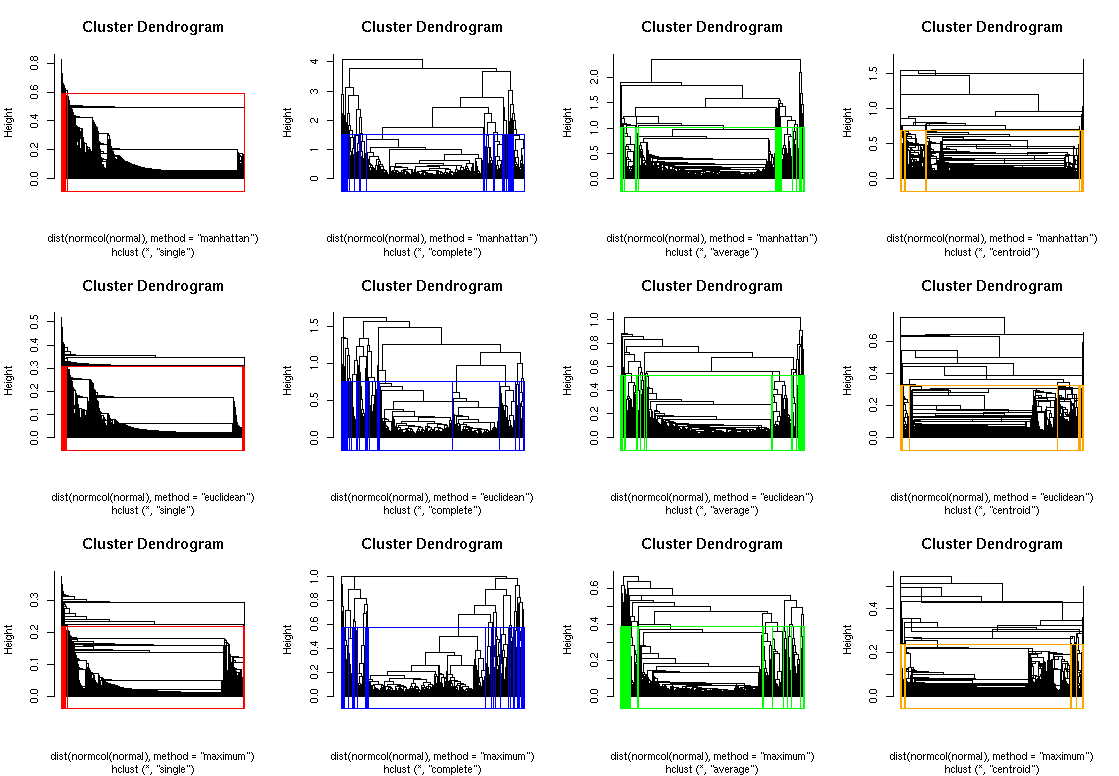
\includegraphics[angle=90, scale=0.55]{Chapter2/treetor_hc.png}
\caption{Hierarchical clustering for the twelve trees
obtained from clustering of torsion angles of the large subunit of 
the ribosome (PDB-ID:1jj2). We have colored a box around branches for the
case where the height of each tree has 36 branches.}
\label{fig:hclus}
\end{figure}

\begin{figure}[htbp]
\centering
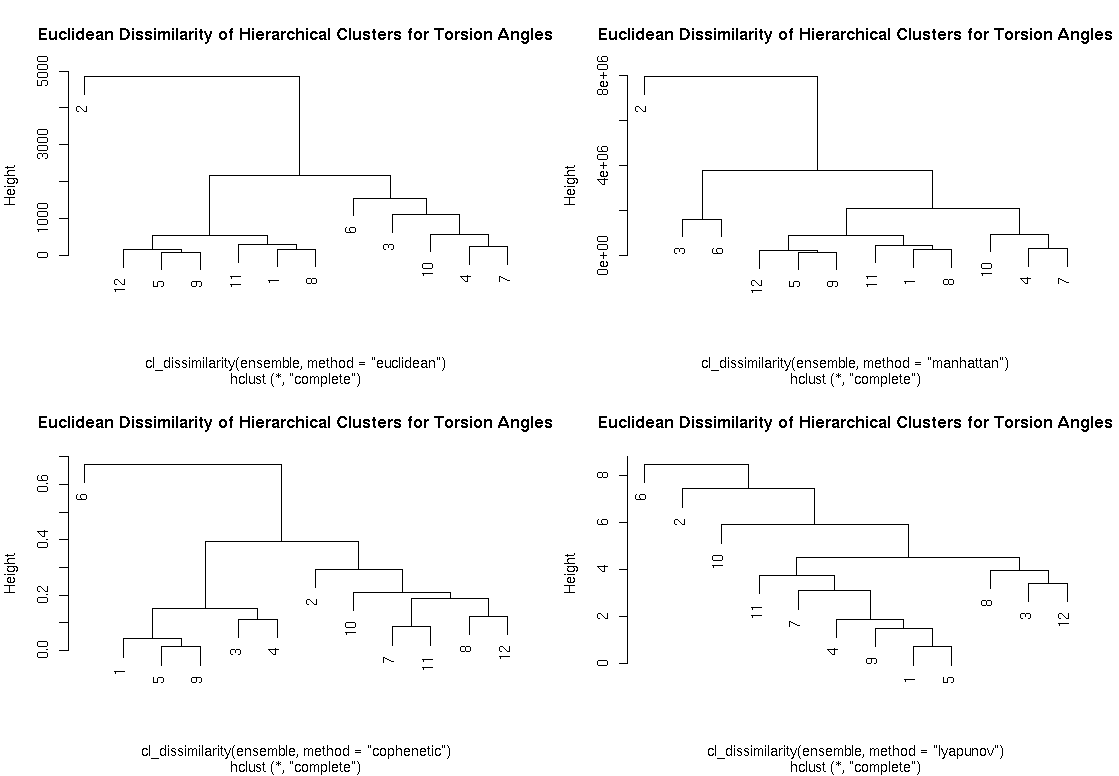
\includegraphics[angle=90, scale=0.60]{Chapter2/clusdissimtor_hc.png}
\caption{Cluster dissimilarities for the 12 combinations of 
metrics and methods used to obtain hierarchical clusterings of the 2753 
heptadimensional torsion  angle vectors of 23S rRNA.}
\label{fig:clusdissim}
\end{figure}


\section{Base-step Parameters}

To our  knowledge there has  been no classification of rigid-body
base-step  parameters for RNA structures deposited at  the
PDB \footnote{The effort of putting together a database for such effort
could be an  interesting project to be considered.}.   It is important
to note here that in  crystal structures, RNA bases are determined more
accurately  than  backbone  torsion  angles,  as  has  been  shown  by
Richardson  and collaborators from  analysis of  van der  Waals steric
clashes.   This can  be seen  more clearly  in Figure~\ref{fig:murray},
reproduced from Richardson's work \cite{murray2003}, where the red
and orange dots  in the backbone atoms region  denote steric clashes and
the green  and yellow  dots in  the base atoms  region denote  very good
agreement with expected van der Waals distances.

\begin{figure}[htbp]
 \centering
 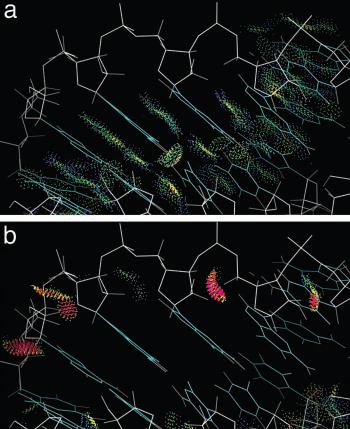
\includegraphics[scale=0.5]{Chapter2/murray2003.png}
 \caption{Figure taken from  Richardson et al. \cite{murray2003} where
 the  blue and  green dots  in  a) mean  very accurate  van der  Waals
 distances, and  in b)  the red and  orange dots mean  steric clashes,
 that is, distances outside the acceptable van der Waals range.}
 \label{fig:murray}
\end{figure}

\subsection{Combining Fourier Averaging Results and Clustering Analysis}
Using the coordinates files of 20 rRNA structures provided by 
Schneider at al.\cite{schneider2004}  we have
used standard clustering analysis (CA) techniques to classify a set of
non-ARNA base-steps  using, rather than the torsion  angles space, the
base-step  parameters space, that  is, three  translational parameters
(Shift$D_x$, Slide$D_y$,  Rise$D_z$), and three  rotational parameters
(Tilt$\tau$,  Roll$\rho$, Twist$\omega$), which  are described  by the
hexaparametric vector $\nu$:

\begin{gather}
 \nu = (D_x, D_y, D_z, \tau, \rho, \omega)
\end{gather}

The     results      illustrated     in     Figures~\ref{fig:eucl_cons}
and~\ref{fig:nonAclus} were  obtained   by   performing  clustering
analysis  and  consensus  clustering  on  20  structures  provided  by
Schneider et  al.  \cite{schneider2004}. These  twenty structures were
obtained  by  Schneider applying  a  Fourier  averaging technique  and
lexicographical  clustering  to  torsion  angles  of  23S  rRNA.   The
methodology  we  used follows  that  used  by  others to  recover  the
periodic table  classification from multidimensional  property vectors
for  elements \cite{restrepo2004,  restrepo2006}. Table~\ref{tab:nonA}
shows the residue  numbers of bases from 23S rRNA  which belong to the
main  categories   of  Figure~\ref{fig:nonAclus}.   To   decide  which
residues of  23S rRNA belonged to  the non-Atype clusters,  a root mean
squared  deviation (RMSD) of  15  or  less  was required  between  step
parameter vectors of  23S rRNA and the mean  parameter vectors for the 
four non-Atype groups identified.

\begin{figure}[htbp]
 \centering
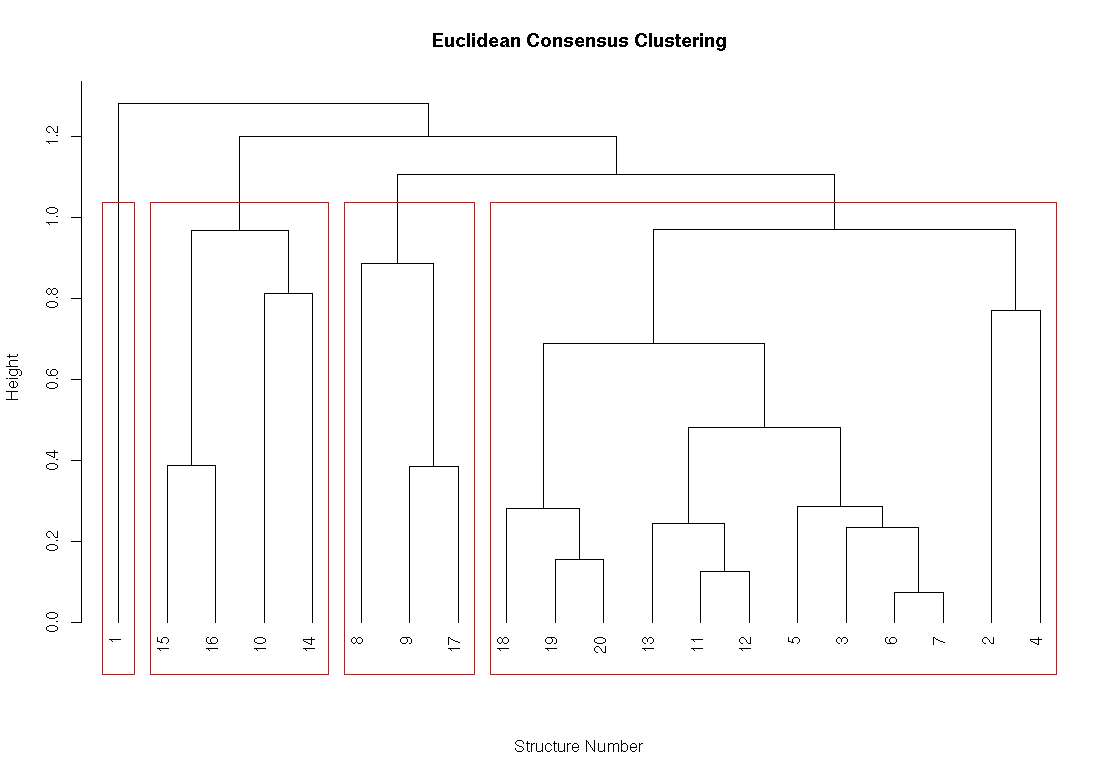
\includegraphics[angle=90, scale=0.6]{Chapter2/eucli_cons_nonA-RNA.png}
\caption{Dendrogram showing the results  of consensus clustering of 20
non-Atype  rRNA  dinucleotides   according  to  their  hexadimensional
base-step parameter vectors.}
 \label{fig:eucl_cons}
\end{figure}

\begin{figure}[htbp]
 \centering
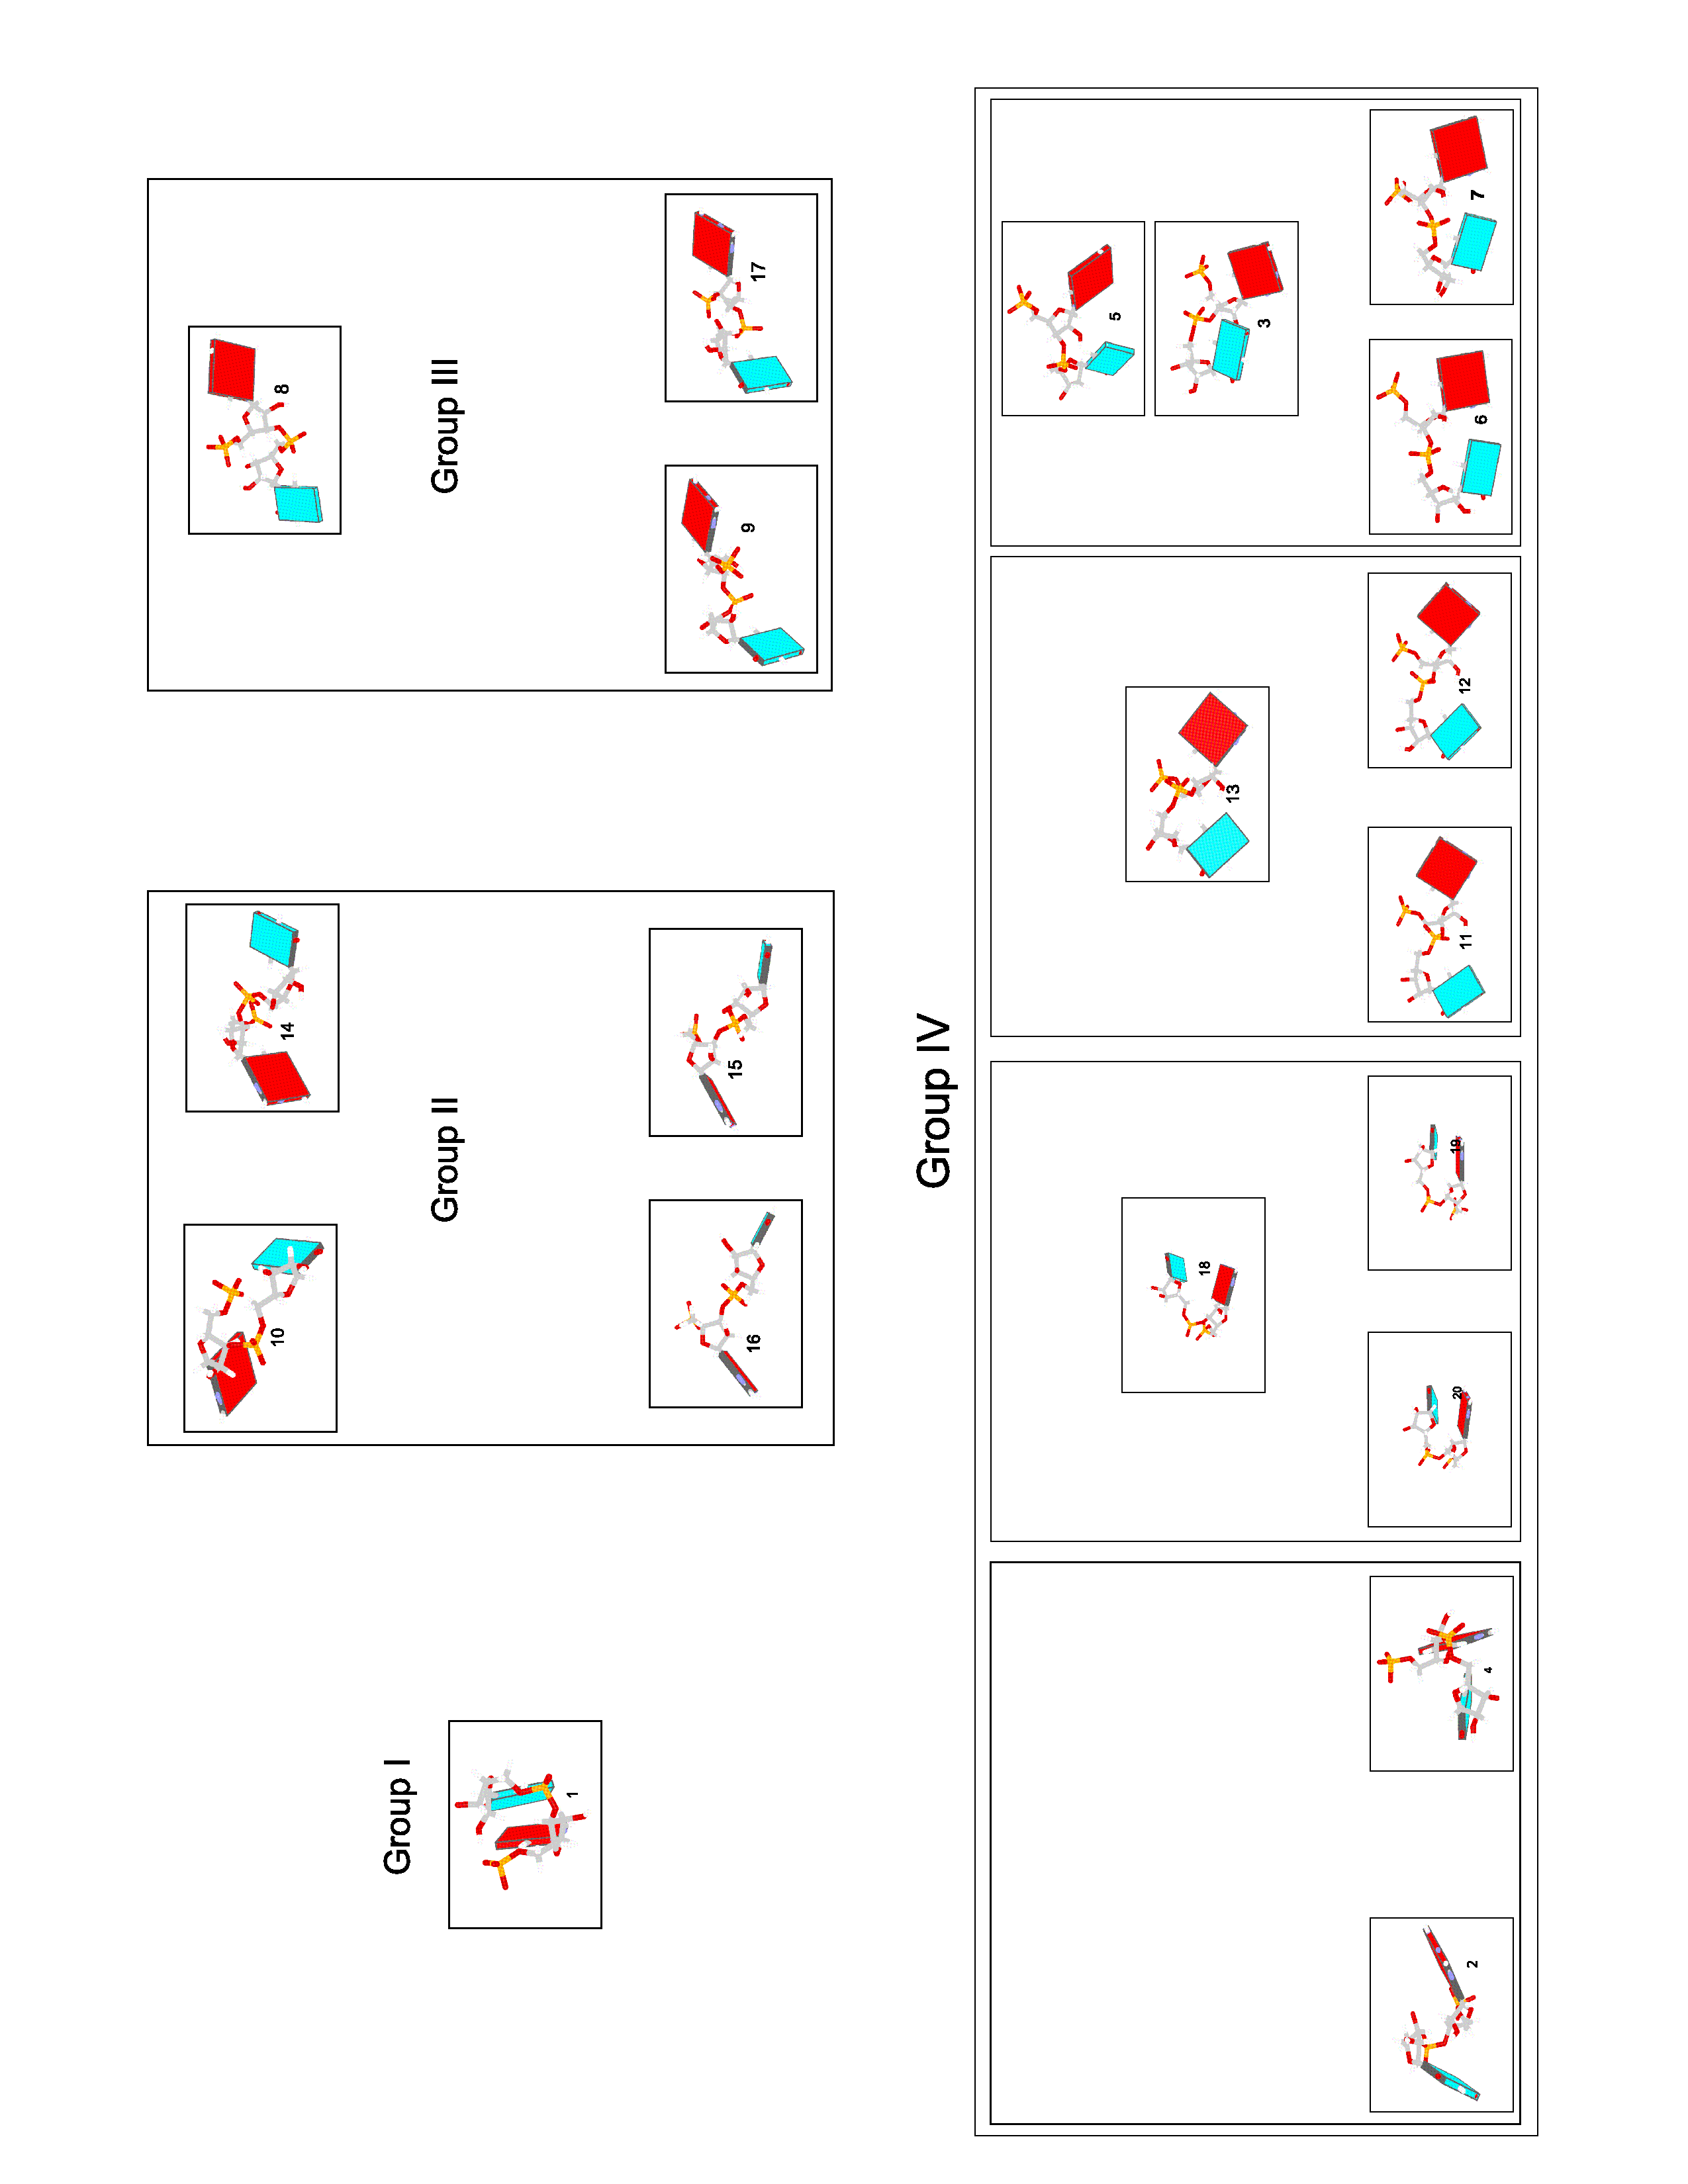
\includegraphics[angle=0, scale=0.8]{Chapter2/Clustered.png}
 \caption{rRNA dinucleotide structures organized by clusters obtained from
consensus clustering of their hexadimensional base-step parameter vectors.}
 \label{fig:nonAclus}
\end{figure}

\begin{table}[htbp]
\begin{center}
{\footnotesize
\begin{tabular}{p{3cm}|p{1,3cm}|c|c|p{3cm}|p{3cm}}
\hline
\bf{Total Number of Nucleotides} & \bf{RMSD Limit} & \bf{Group} & \bf{Base-steps}
& \bf{Base-step Residue Number} & \bf{Overlaps} \\ \hline
2754 & $ < 15$ & I & 3 & 892, 2006, 2390 &  \\ \hline
 &  & II & 5 & 459, 1279, 1653, 1919, 2302 &  \\ \hline
 &  & III & 1 & 2109 &  \\ \hline
 &  & IV & 35 & 79, 112, 128, 190, 213, 269, 358, 434, 488, 564, 706,
 720, 775, 867, 966, 1292, 1503, 1543, 1614, 1766, 1874, 1908, 1971, 
 2017, 2257, 2427, 2516, 2540, 2755, 2782, 2810, 2826, 2874, 2882, 2913 &  \\ \hline
 &  & IVa & 1 & 882 &  \\ \hline
 &  & IVb & 807 &  &  \\ \hline
 &  & IVc & 9 & 306, 789, 854, 880, 1107, 1192, 1493, 1818, 2005 &  \\ \hline
 &  & IVd & 35 & 175, 213, 246, 264, 304, 358, 464, 518, 531, 534,
 588, 795, 938, 1214, 1231, 1316, 1340, 1370, 1605, 1745, 1766, 
 1971, 1976, 2010, 2017, 2291, 2320, 2428, 2469, 2481, 2516, 2532, 
 2755, 2826, 2882 & Only IVd with IV (213, 358, 1766, 1971, 2017, 
 2516, 2755, 2826, 2882) \\ \hline
\end{tabular}
}
\caption{Residue numbers for base-steps  with RMSD values less than 15
between  the  reference base-step  vectors  from  the  four groups  of
non-A-type  RNA dinucleotide conformations  and all  base-step vectors
found  in  the 23S  strand  of  \textit{Haloarcula marismortui}  large
ribosomal subunit.}
\label{tab:nonA}
\end{center}
\end{table}


\subsection{Partitional Clustering for Rigid Body Parameters}

The same type of analysis that has been carried out for torsion angles
can  also  be  carried  out   for  rigid  body  parameters,  that  is,
partitional  clustering, and  hierarchical  clustering, are used  as 
standard statistical  analysis methods  to analyze  our set  of  2753 
base-step parameter vectors.  For the  partitional clustering case, 
again, there is no known number of clusters in which the data must
group, therefore we've  calculated the  within clusters  sum  of
squares and also  the
average silhouette widths, for a particular selection of the number of
partitions of the data for $k=[2-80]$.  From figure~\ref{fig:wssSteps}
we can't conclude  much. We see that the value  of the within clusters
sum  of squares  becomes constant  around  $k=47$ and  there´s also  a
change of  curvature around  $k=13$.  For the  case where  the average
silhoutte width has been computed, that is, figure~\ref{fig:aswSteps},
we see that  the maximum is for $k=2$, and  there are some interesting
maxima at  $k=9,12$.  Now that  we have a  clue as to which  number of
partitions the data  optimally has we have plotted  the k-means results
for $k=13$ and $k=47$ in Figures  bla and bla, and the PAM results for
$k=2, 9, 12$ in Figure bla.


We have  also prefiltered  the data according  to the 16  possible RNA
base steps, that is,  AA, AG, GA, GG, UU, UC, CU,  CC, UA, UG, CA, CG,
AU, AC,  GU, and  GC.  Tables showing  how many  representatives steps
there are  belonging to  non-helical, helical, and  watson-crick sets,
will be later included and discussed here.

\begin{figure}[htbp]
\centering
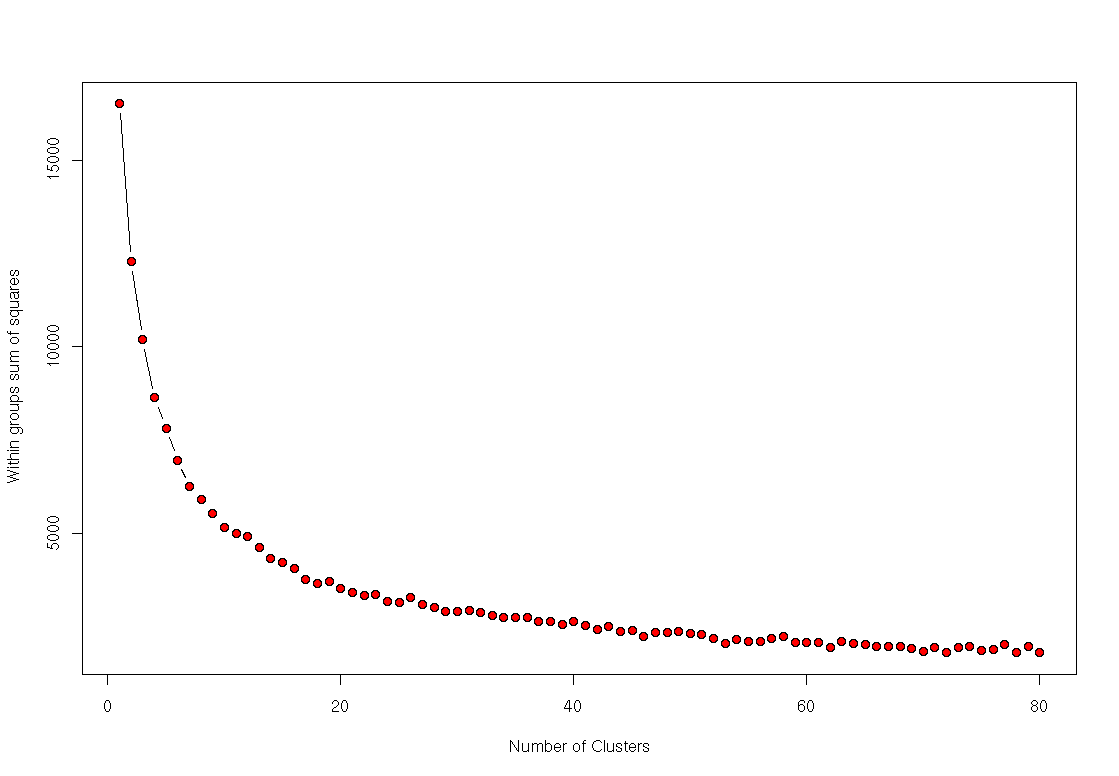
\includegraphics[angle=0, scale=0.40]{Chapter2/hartigan_nuclu_steps_b.png}
\caption{Sum of all within clusters sum of squares against number of clusters.}
\label{fig:wssSteps}
\end{figure}

\begin{figure}[htbp]
 \centering
 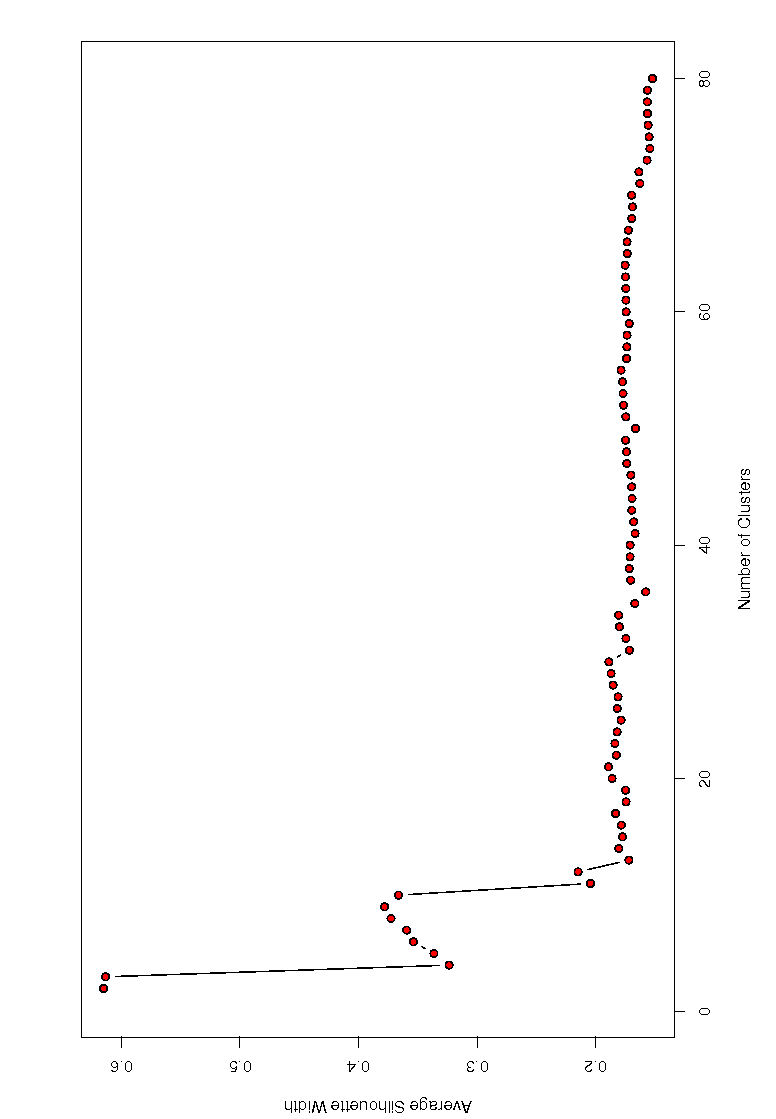
\includegraphics[angle=270, scale=0.50]{Chapter2/pam_asw_2_80_steps.png}
 \caption{Average silhouette width against number of clusters.}
 \label{fig:aswSteps}
\end{figure}



\subsection{Hierarchical Clustering for Rigid Body Parameters}

Also as has been carried out for torsion angles, hierarchical clustering has
also been performed on rigid body parameters, the results are yet to be
included here. A cluster dissimilarity tree can be seen in
Figure~\ref{fig:clusdis} for the 12 trees resulting from the four clustering
methods and three distance definitions used to cluster the base step data.

\begin{figure}[htbp]
\centering
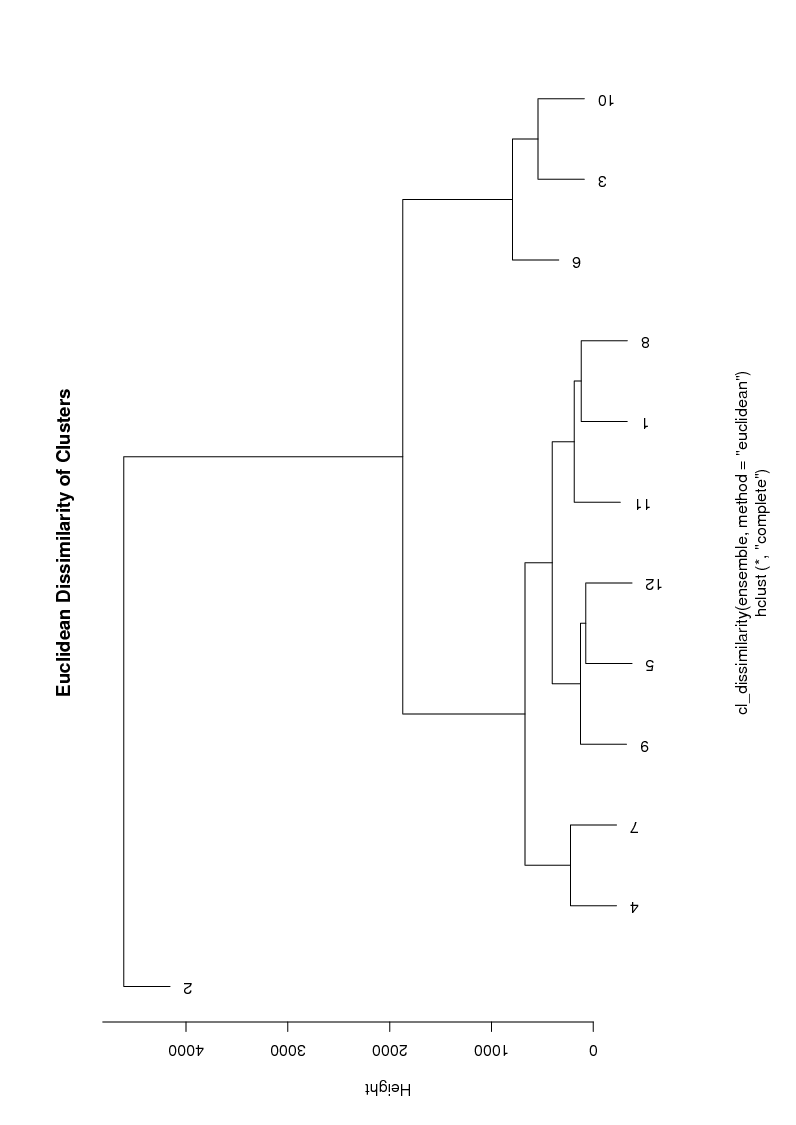
\includegraphics[scale=0.60]{Chapter2/clussdissim.png}
\caption{Cluster dissimilarities for the twelve hierarchical trees
  obtained from clustering of the six-dimensional base-step parameters
obtained from the large subunit of the ribosome (PDB-ID:1jj2)}
\label{fig:clusdis}
\end{figure}


\section{RNA Conformations}
There are two main RNA conformations, A-RNA ,and A'RNA, and maybe even a
third unconfirmed one A"RNA \cite{saenger1984}.
Their values for their standard torsion angles and step parameters can be seen
in Tables~\ref{tab:tor_conf} and ~\ref{tab:step_conf} 

\begin{table}[htbp]
\begin{center}
{\small
\begin{tabular}{c|c|c|c|c|c|c|c|c}
\hline
\bf{Structure Name} & $\alpha$ & $\beta$ & $\gamma$ & $\delta$ & $\epsilon$
& $\zeta$ & $\chi$ & \bf{Reference} \\ \hline
A-RNA & -68.9 & 179.5 & 54.5 & 82.2 & -153.9 & -70.8 & -161.1 & Arnott \\ \hline
A'-RNA & -70.0 & 176.6 & 60.8 & 76.7 & -153.4 & -69.4 & -163.4 & Arnott \\ \hline
AII-RNA & -65.0 & 175.1 & 52.9 & 81.1 & -166.0 & -68.0 & -157.0 & Schneider \\ \hline
\end{tabular}
}
\caption{Base step torsion angles for the different known RNA conformations.}
\label{tab:tor_conf}
\end{center}
\end{table}

\begin{table}[htbp]
\begin{center}
{\small
\begin{tabular}{p{2cm}|c|c|c|c|c|c|c}
\hline
\bf{Structure Name} & Shift ($D_x$) & Slide ($D_y$) & Rise ($D_z$) & Tilt
($\tau$) & Roll ($\rho$) & Twist ($\Omega$) & \bf{Reference} \\ \hline
A-DNA & 0.36 & -1.39 & 3.29 & 2.46 & 12.50 & 30.19 & \\ \hline
B-DNA & 0.44 & 0.47 & 3.33 & 4.63 & 1.77 & 35.67 & \\ \hline
A-RNA & -0.08 & -1.48 & 3.30 & -0.43 & 8.64 & 31.57 & Arnott \\ \hline
A'-RNA & 0.05 & -1.88 & 3.39 & -0.12 & 5.43 & 29.52 & Arnott \\ \hline
AII-RNA & 1.01 & -2.52 & 3.33 & 2.94 & 9.75 & 25.12 & Schneider \\ \hline
\end{tabular}
}
\caption{Base step parameters for the different known RNA
  conformations. Notice that the base step parameters are for single
  bases rather than base-pairs.}
\label{tab:step_conf}
\end{center}
\end{table}




\begin{figure}[htbp]
\centering
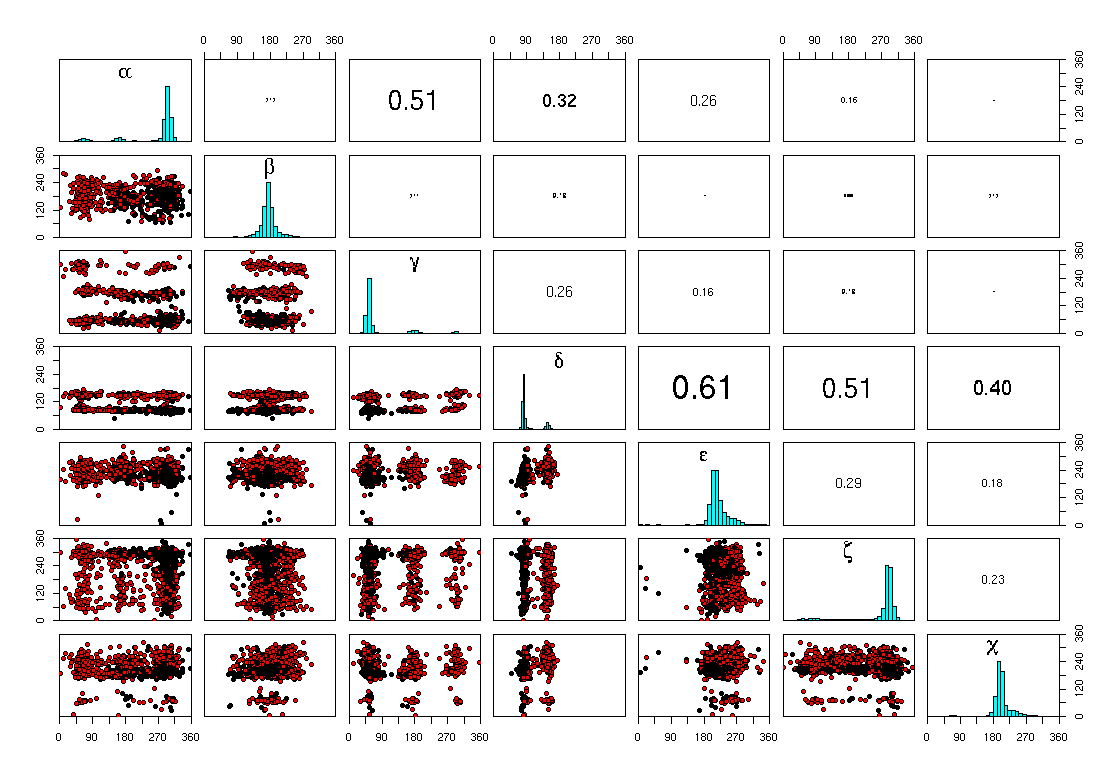
\includegraphics[angle=90, scale=0.50]{Chapter2/hartigan_tor_b.png}
\caption{
K-means of torsion  angle vectors of 2753 dinucleotide steps
present in  23S rRNA using the  \textit{Hartigan-Wong} algorithm.  The
number  of  partitions  is  \textbf{2}.   The  upper  diagonal  matrix
displays the values  of the linear correlation coefficient  $r$, and a
histogram showing  the torsion angle distribution is rendered  in the
diagonal.}
\label{fig:hartigan}
\end{figure}

\begin{figure}[htbp]
\centering
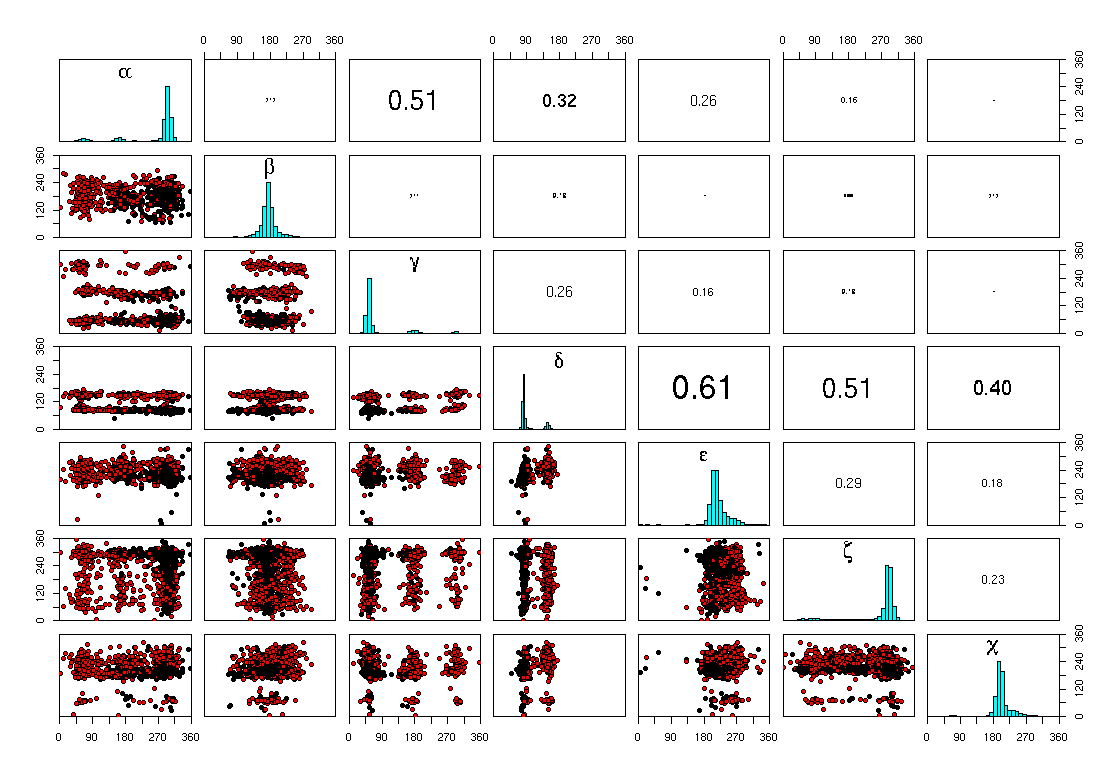
\includegraphics[angle=90, scale=0.50]{Chapter2/lloyd_tor_b.png}
\caption{
K-means of torsion  angle vectors of 2753 dinucleotide steps
present in  23S rRNA using the  \textit{Lloyd} algorithm.  The
number  of  partitions  is  \textbf{2}.   The  upper  diagonal  matrix
displays the values  of the linear correlation coefficient  $r$, and a
histogram showing  the torsion angle  distribution is rendered  in the
diagonal.}
\end{figure}

\begin{figure}[htbp]
\centering
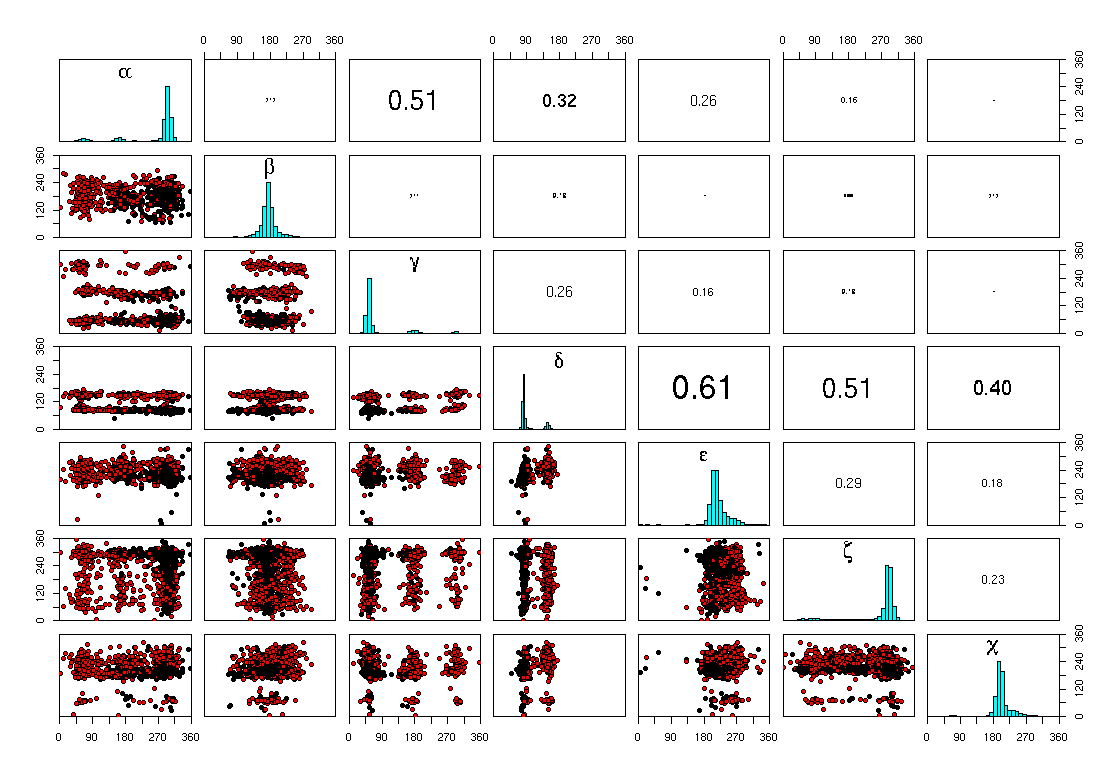
\includegraphics[angle=90, scale=0.50]{Chapter2/forgy_tor_b.png}
\caption{
K-means of torsion  angle vectors of 2753 dinucleotide steps
present in  23S rRNA using the  \textit{Forgy} algorithm.  The
number  of  partitions  is  \textbf{2}.   The  upper  diagonal  matrix
displays the values  of the linear correlation coefficient  $r$, and a
histogram showing  the torsion angle  distribution is rendered  in the
diagonal.}
\end{figure}

\begin{figure}[htbp]
\centering
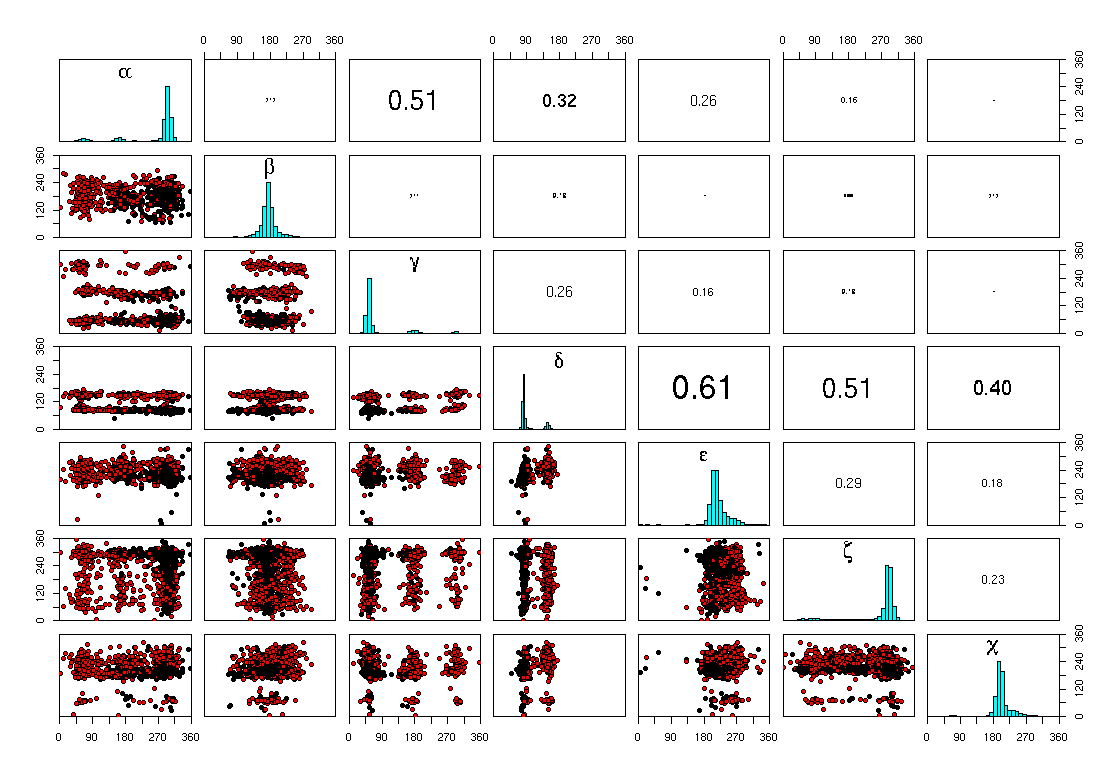
\includegraphics[angle=90, scale=0.50]{Chapter2/macqueen_tor_b.png}
\caption{
K-means of torsion  angle vectors of 2753 dinucleotide steps
present in  23S rRNA using the  \textit{McQueen} algorithm.  The
number  of  partitions  is  \textbf{2}.   The  upper  diagonal  matrix
displays the values  of the linear correlation coefficient  $r$, and a
histogram showing  the torsion angle  distribution is rendered  in the
diagonal.}
\label{fig:macqueen}
\end{figure}




This chapter deals with how starting from a backbone based view of
RNA, we can make an interpretation at the step level using the block model.
\section{Consensus Clustering of Single Stranded Base Step Parameters}

\section{Four Major Non-ARNA Step Groups in the Ribosome}

\bibliography{biblio}

